\documentclass{beamer}
\usepackage{listings}
\lstset{
%language=C,
frame=single, 
breaklines=true,
columns=fullflexible
}
\usepackage{subcaption}
\usepackage{url}
\usepackage{tikz}
\usepackage{tkz-euclide} % loads  TikZ and tkz-base
%\usetkzobj{all}
\usetikzlibrary{calc,math}
\usepackage{float}
\newcommand\norm[1]{\left\lVert#1\right\rVert}
\providecommand{\pr}[1]{\ensuremath{\Pr\left(#1\right)}}
\renewcommand{\vec}[1]{\mathbf{#1}}
\usepackage[export]{adjustbox}
\usepackage[utf8]{inputenc}
\usepackage{amsmath}
\usetheme{Boadilla}

\title{Deduction from Conditional Knowledge on Bayesian Networks with Interval Probability Parameters}
\author{Tanmay Goyal - AI20BTECH11021}

\date{}

\begin{document}

\begin{frame}
\titlepage
\end{frame}
\begin{frame}
\frametitle{Bayesian networks}
\begin{columns}
\begin{column}{0.5\textwidth}
\begin{figure}
\begin{flushleft}
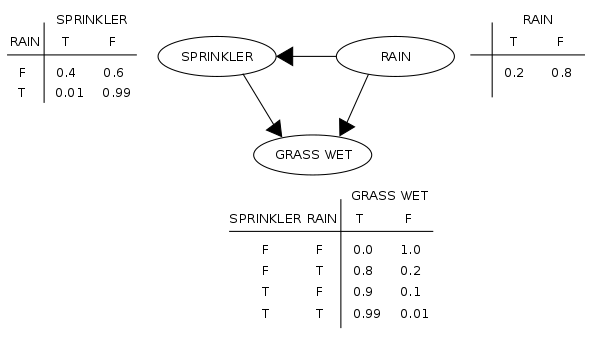
\includegraphics[width=\columnwidth]{Figures/Bayesian Network.png}
\end{flushleft}
\end{figure}
\begin{enumerate}
    \item Directed Acyclic Graph (DAG)\\
    \item Represents Probabilistic Relationships
\end{enumerate}
\end{column}
\begin{column}{0.5\textwidth}
Find Probability that it is raining, given grass is wet?
\begin{align}
    \pr{R = T | G = T}\\
    = \frac{TTT + TFT}{TTT + TFT + FTT + FFT}
\end{align}
\end{column}
\end{columns}

\end{frame}

\begin{frame}[fragile]
\frametitle{Logic Vs Probability}

\begin{flushleft}
\begin{enumerate}
    \item Boolean Logic: $b \rightarrow a $, "if b, then a", \pr{a|b}\\
    \item Classical Logic: \pr{b\rightarrow a} = \pr{a|b} + \pr{b'}\pr{a' | b} \geq \pr{a|b}\\
    \begin{align}
         = \frac{\pr{a,b}+ \pr{b'}(\pr{b} - \pr{a,b})}{\pr{b}}\\
         = \pr{a,b} + \pr{b'}
    \end{align}
        \end{enumerate}
          \end{flushleft}
    \begin{flushleft}
    \begin{enumerate}
     \setcounter{enumi}{2}
      \item {Lewis' Theorem:} cannot equate the conditional probability $\pr{A|B}$ with the probability of conditional event, $B\rightarrow A$, except for a trivial set of events\\
      \item {Conditional Event Algebra (CEA):} Unlike Boolean Algebra, allows defining $\pr{B\rightarrow A} = \pr{A|B}$ over a broad range of conditions
      \item CEA allows generalisation of Boolean Algebra to conditional events, while maintaining compatibility of standard and conditional probability
    \end{enumerate}
\end{flushleft}
\end{frame}

\begin{frame}[fragile]
\frametitle{Interval Probability and Higher Order Logic}
\begin{enumerate}
    \item A {p-probability interval} for $\theta$ is an interval $[a,b]$ with $\pr{a \leq \theta \leq b} = p$, which can be $\sum_{a\leq \theta_i \leq b} \pr{\theta_i}$ or $\int_a^b f(\theta)\,d\theta$\\
    \item \alert{Interval Parameters:} $a$ and $b$
    \item {Higher- Order Logic:} if $b_1$ then $a_1$,if $b_2$ then $a_2 \ldots$ then if $c$ then $d$\\
    \item $\pr{c|(a|b)} \neq \pr{c|(a'\cup b)}$\\
    \item The existing definitions and concepts of interval probability do not apply to conditional probability, and cannot be used to draw inferences from higher- order conditionals using BNs.\\
    \item {Proposal:} Bayesian higher- order probabilistic reasoning approach with interval probability parameters, combining CEA and weak conditional probability.
\end{enumerate}
\end{frame}

\begin{frame}[fragile]
\frametitle{Conditional Event Algebra}
\begin{flushleft}
\begin{enumerate}
    \item Mathematically modelling conditionals as conditional events. Express probability weight of "$b \rightarrow a$" in terms of \pr{a|b}\\
    \item Let $(\Omega, B, P) $ be a standard probability space such that $\Omega$ represents the Sample Space, $B$ represents a definite event, and $P$ a certain probability measure:
    \begin{enumerate}
        \item $P(\Omega) =1$\\
        \item $P(b_1 \cup b_2 \cup \ldots  + b_j + \ldots) = P(b_1) + P(b_2) \ldots + P(b_j) + \ldots$ for mutually exclusive $b_i$s\\
        \item The set of all conditional events is Boolean Algebra with connectives $\wedge, \vee$ and ' \\
        \item Any probability measure $P$ defined on events  of $\Omega$ can be extended a probability measure $P_0$ on conditional events such that $P_0(a|b) = P(a|b)$, i.e conditional probability is a true probability measure on conditional events.
        
    \end{enumerate}
\end{enumerate}
\end{flushleft}

\end{frame}

\begin{frame}{fragile}
\frametitle{Conditional Event Algebra}

\begin{flushleft}
    \begin{enumerate}
        \item Given normal events $a$ and $b$, we define an extended probability space $(\Omega_0 , B_ 0 , P_0)$, such that, $\Omega_ 0 = \Omega \times \Omega \times \ldots$, $B_ 0 = B \times B \times \ldots$, and $B_0$ being a Boolean Algebra extension. Then,
        {\small
        \begin{align}
            (a|b) = ((a\wedge b)\times \Omega_0) \vee (b'\times (a\wedge b)\times \Omega_0) \vee (b'\times b'\times (a\wedge b)\times \Omega_0) \ldots
        \end{align}
        }
        \item Define $f: B \times B \rightarrow B_0$ as:
        \begin{align}
            f(a,b) = ab \vee (b'\times ab) \vee (b'\times b'\times ab) \ldots\\
            \label{CEAeqn}
            P_0(f(a,b)) = P_0(ab)  + P_0(b'\times ab) + P_0(b'\times b'\times ab) \ldots\\
            P_0(f(a,b)) = P(ab) \sum P(b')^j\\
            = P(a|b)
        \end{align}
    \end{enumerate}
\end{flushleft}
    
\end{frame}

\begin{frame}
    \frametitle{Probability logic reasoning on Bayesian Networks}
    \begin{flushleft}
       If if $b_1$ then $a_1$ and if $b_2$ then $a_2 \ldots$ then if $d$ then $c$ can be expressed as:
        \begin{align}
            G = [(a|b)_j;(c|d)]\\
            A(G) = \cap \{a_j b_j ,  a_j' b_j, b_j' \} \cap \{cd,c'd,d'\} \\
            = \{\omega_1 , \omega_2 ,\ldots \omega_{m}\}
        \end{align}
        From \eqref{CEAeqn}
        \begin{align}
            f(a_j,b_j,c,d) = \vee (\omega_j)\\
            \pr{(a|b)_j;(c|d)} = \pr{A(G)} 
            = P_0(f(a_j,b_j,c,d)) \\
            = \sum \pr{w_j}
        \end{align}
  \end{flushleft}
\end{frame}


\begin{frame}
    \frametitle{Interval Probability}
    \begin{enumerate}
        \item $U$- universe, $S$-subset of $U$. $S$ is called an interval value if $v_1,v_2,v_3 \in U$ and $v_1 \leq v_2 \leq v_3$, and $v_1, v_3 \in S$ implies $v_2 \in S$ 
        \newline
        \item Let $b$ be a random event, then \alert{lower and upper probabilities}, written as \alert{$L(b)$ and $U(b)$}, are given by: ($x_i$ denotes a sample from sample space $\Omega$)
        \begin{enumerate}
            \item $L(b) = \sum \pr{x_i}$ for $x_i$ in $b$
 
            \item $U(b) = \sum \pr{x_i}$ for $x_i \cap b \neq \phi$
            \newline
        \end{enumerate}
        
        \item $L(a) \leq \pr{a} \leq U(a)$
    
    \end{enumerate}
\end{frame}

\begin{frame}
    \frametitle{Interval Probability}
    \begin{enumerate}
          \item $L(a|b) = inf \frac{\pr{a \cap b}}{\pr{b}}$ and $U(a|b) = sup \frac{\pr{a \cap b}}{\pr{b}}$ where $pr(b) \neq 0$
          \newline
          \item Bound limited weak conditional probabilities: $BL(a|b)$ and $BU(a|b)$
    
          \begin{enumerate}
              \item  If $ L(a) \leq L(a|b) \leq U(a|b) \leq U(a)$, then
$BL(a|b)=max\{EL(a|b), L(a)\}$ and $BU(a|b)=min\{EU(a|b),
U(a)\}$
\newline
\item If $ L(a|b) \leq L(a) \leq U(a) \leq U(a|b)$, then
$BL(a|b)=min\{EL(a|b), L(a)\}$ and $BU(a|b)=max\{EU(a|b),
U(a)\}$
\newline
          \end{enumerate}
  \newline
          \item $BL(a|b) \leq \pr{a|b} \leq BU(a|b)$
    \end{enumerate}
\end{frame}

\begin{frame}
    \frametitle{Multiplication rules}
    \begin{enumerate}
        \item $L(abc) \approx BL(abc) = L(a)BL(b|a)BL(c|ab)$
        \newline 
        \item $U(abc) \approx BU(abc) = U(a)BU(b|a)BU(c|ab)$
    \end{enumerate}
\end{frame}

\begin{frame}
    \frametitle{Probability logic reasoning on Bayesian Networks}
    \begin{align}
        BL(\omega_j) \leq \pr{\omega_j} \leq BU(\omega_j)\\
         \sum BL(\omega_j) \leq  \sum \pr{\omega_j} \leq \sum BU(\omega_j)\\
         \sum BL(\omega_j) \leq \pr{(a|b)_j;(c|d)} \leq \sum BU(\omega_j)
    \end{align}
    \underline{Logic:}
    Conditional Events $\longrightarrow$ Joint events $\longrightarrow$ Multiplication rule 
\end{frame}
\begin{frame}
    \frametitle{Example}
    \begin{align}
        \pr{d|(b|a),(c|a)} \\
        G = [(b|a), (c|a) ; (d|\Omega)]\\
        A(G) = \{ba,b'a,a'\} \wedge \{ca,c'a,a'\} \wedge \{d\Omega , d'\Omega , \phi\}
\end{align}
\begin{center}
    \begin{tabular}{|c|c|}
\hline
     $abcd$ & $\omega_1$  \\
     \hline
     $ab'cd$ & $\omega_2$  \\
     \hline
      $abc'd$ & $\omega_3$  \\
     \hline
      $ab'c'd$ & $\omega_4$  \\
     \hline
      $a'd$ & $\omega_5$  \\
     \hline
      $abcd'$ & $\omega_6$  \\
     \hline
      $ab'cd'$ & $\omega_7$  \\
     \hline
      $abc'd'$ & $\omega_8$  \\
     \hline
      $ab'c'd'$ & $\omega_9$  \\
     \hline
      $a'd'$ & $\omega_{10}$  \\
     \hline
\end{tabular}
\end{center}
\end{frame}

\begin{frame}
\frametitle{Example}
    \begin{columns}
\begin{column}{0.5\textwidth}
\begin{figure}
\begin{flushleft}
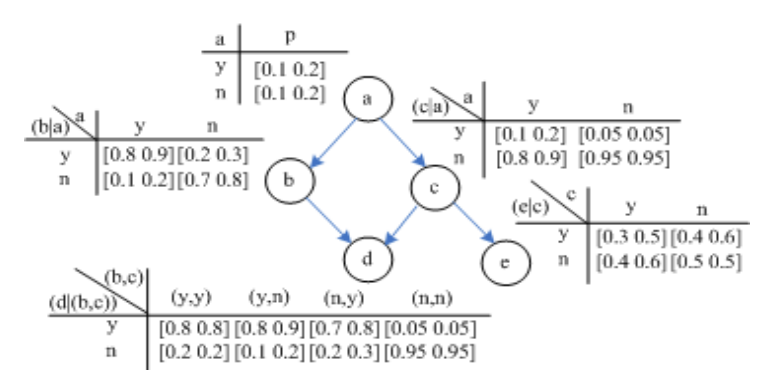
\includegraphics[scale = 0.245]{Figures/Example.png}
\end{flushleft}
\end{figure}
\end{column}
\begin{column}{0.5\textwidth}
{\small
\begin{align}
    BL(\omega_1) = BL(abcd)\\
    = L(a)BL(b|a)BL(c|a)BL(d|bc)\\
    = 0.1 \times 0.8 \times 0.1 \times 0.8 \\
    = 0.0064
    \end{align}\
    \begin{align}
        BU(\omega_1) = BU(abcd)\\
    = U(a)BU(b|a)BU(c|a)BU(d|bc)\\
    = 0.2 \times 0.8 \times 0.2 \times 0.9 \\
    = 0.0288
\end{align}
}
\end{column}
\end{columns}
\end{frame}


\begin{frame}
\frametitle{Example}
    \begin{center}
    \begin{tabular}{|c|c|c|c|}
\hline
      & & BL(.) & BU(.)\\
      \hline
     $abcd$ & $\omega_1$ & 0.0064 & 0.0288  \\
     \hline
     $ab'cd$ & $\omega_2$ & 0.0007 & 0.0064 \\
     \hline
      $abc'd$ & $\omega_3$ & 0.0512 & 0.1458 \\
     \hline
      $ab'c'd$ & $\omega_4$ & 0.0004 & 0.0018  \\
     \hline
      $a'd$ & $\omega_5$ & 0.0217 & 0.0677  \\
     \hline
      $abcd'$ & $\omega_6$ & 0.0016 & 0.0072 \\
     \hline
      $ab'cd'$ & $\omega_7$ & 0.0020 & 0.0024 \\
     \hline
      $abc'd'$ & $\omega_8$ & 0.0064 & 0.0324  \\
     \hline
      $ab'c'd'$ & $\omega_9$ & 0.0076 & 0.0342 \\
     \hline
      $a'd'$ & $\omega_{10}$ & 0.0660 & 0.1588   \\
     \hline
     & $\sum \omega_j$& 0.1766 & 0.4855\\
     \hline
\end{tabular}
\end{center}
The probability of G is estimated to be between [0.1766,0.4855]
\end{frame}

\end{document}